\begin{comment}
\documentclass[lang=cn,10pt,green]{elegantbook}
\usepackage{subcaption} % 引入 subfigure 宏包
\title{2025年中级宏观经济学笔记}
\subtitle{授课: 余昌华老师}

\author{徐靖}
\institute{PKU}
\date{Febuary 28, 2025}
\bioinfo{声明}{请勿用于个人学习外其他用途!}

\extrainfo{个人笔记, 如有谬误, 欢迎指正! 联系方式 : 2200012917@stu.pku.edu.cn}

\setcounter{tocdepth}{3}

\logo{logo-blue.png}
\cover{cover.jpg}

% 本文档命令
\usepackage{array}
\newcommand{\ccr}[1]{\makecell{{\color{#1}\rule{1cm}{1cm}}}}

% 修改标题页的橙色带
% \definecolor{customcolor}{RGB}{32,178,170}
% \colorlet{coverlinecolor}{customcolor}

\begin{document}

\maketitle
\frontmatter

\tableofcontents

\mainmatter
%\end{comment}

\chapter{The Data of Macroeconomics}
\begin{introduction}[Keywords]
    \item GDP gross domestic product  国内生产总值
    \item CPI consumer price index 消费者物价指数
    \item Expenditure 支出
\end{introduction}
\section{Gross Domestic Product: Expenditure and Income}
\subsection{GDP}
\begin{definition}
    \textbf{Value added} 增加值 : 产出的市场价值减去用于生产该产出的中间产品的市场价值
\end{definition}

\begin{figure}[htbp]
    \centering
    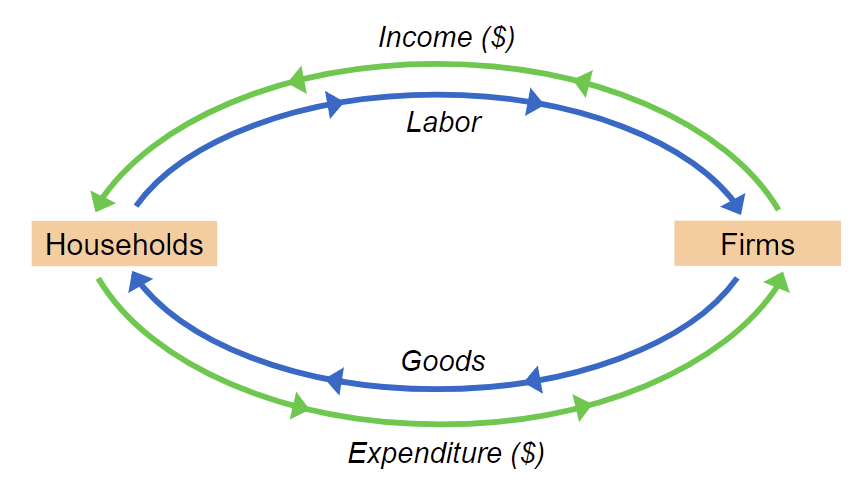
\includegraphics[width=0.6\textwidth]{image/CircularFIOW.png}
    \caption{循环流动}
\end{figure}
\begin{note}
    支出等于收入,因为买方花费的每一美元都会成为卖方的收入
\end{note}
\begin{definition}
    支出法 GDP = C + I + G + NX 
    \begin{itemize}
        \item C: consumption 消费
        \item I: investment 投资
        \item G: government spending 政府支出
        \item NX: net exports 净出口
        \begin{itemize}
            \item NX = exports - imports 
        \end{itemize}
    \end{itemize}
\end{definition}

\begin{problem}
    Why output = expenditure
\end{problem}
\begin{itemize}
    \item 没有卖出的产品投入库存, 被计算为库存投资
    \item 实际上, 我们假设没有库存投资, 公司买下没卖的产品
\end{itemize}

\subsection{GNP and GDP}
\begin{itemize}
    \item GNP: Gross National Product 国民生产总值, 国民在国内外生产的总值
    \item GDP: Gross Domestic Product 国内生产总值, 国内生产的总值
    \item GNP - GDP = 国际收支, 从国外支付的要素减去向国外支付的要素
\end{itemize}
\begin{note}
国家之间 $GNP - GDP / GDP$ 的比值为正, 说明国家对外资本净收入为正, 反之为负, 美国为正, 中国为负, 冰岛非常低.
\end{note}
\subsection{Real and Nominal GDP}
\begin{itemize}
    \item Nominal GDP: 以当年价格计算的 GDP
    \item Real GDP: 以基年价格计算的 GDP
\end{itemize}
\begin{note}
    目的是抵消通货膨胀的影响, 从而在不同年份比较 GDP 的增长.
\end{note}
\subsection{GDP Deflator}
\begin{definition}
    GDP deflator = $\frac{\text{Nominal } GDP}{\text{Real } GDP} \times 100$
\end{definition}
\begin{note}
    GDP deflator (GDP 平减指数) 反映了物价水平的变化, 也可以用来计算通货膨胀率.
\end{note}

\begin{lemma}
    Percentage change in $XY$ = percentage change in $X$ + percentage change in $Y$
\end{lemma}
\subsection{Chain-weighted real GDP}

\begin{itemize}
    \item 随着时间的推移,相对价格会发生变化,因此基年应定期更新。
    \item \textbf{链式加权实际GDP}
    \begin{itemize}
        \item 链式加权实际GDP每年都会更新基年,因此它比不变价格GDP更准确。
    \end{itemize}

    \item \textbf{不变价格实际GDP}
    
\begin{itemize}
        \item 教科书通常使用不变价格实际GDP,原因如下:
        \begin{itemize}
            \item 两种衡量方法高度相关
            \item 不变价格实际GDP更易于计算
        \end{itemize}
    \end{itemize}
\end{itemize}

\section{Consumer Price Index}
\begin{definition}
    Consumer Price Index (CPI) = $\frac{\text{cost of basket in current year}}{\text{cost of basket in base year}} \times 100$
\end{definition}
\begin{note}
    CPI 反映了消费者购买商品和服务的价格变化, 用来衡量通货膨胀.
\end{note}
\begin{problem}
    Why the CPI may overstate(高估) inflation 
\end{problem}

\begin{itemize}
    \item \textbf{替代偏差}
    \begin{itemize}
        \item CPI 使用固定权重,因此无法反映消费者转向相对价格下降的商品的能力。
    \end{itemize}
    \item \textbf{新商品的引入}
    \begin{itemize}
        \item 新商品的引入使消费者福利增加,实际上提高了美元的实际价值。但由于 CPI 使用固定权重,它并未反映这一变化。
    \end{itemize}
    \item \textbf{变化的未完全测量}
    \begin{itemize}
        \item 质量的提高增加了美元的价值,但这些改进往往未能被完全纳入 CPI 的测量中。
    \end{itemize}
\end{itemize}
\begin{note}
    1995 年, CPI 每年高估了 1.1\% 的通货膨胀率. 现在, CPI 的偏移降到了 1\% 以下.
\end{note}

\subsection{CPI vs GDP deflator}
\begin{itemize}
    \item \textbf{资本品的价格}
    \begin{itemize}
        \item 包含在 GDP 平减指数中(如果在国内生产)
        \item 不包括在 CPI 中
    \end{itemize}

    \item \textbf{进口消费品的价格}
    
\begin{itemize}
        \item 包含在 CPI 中
        \item 不包括在 GDP 平减指数中
    \end{itemize}

    \item \textbf{商品篮子}
    
\begin{itemize}
        \item CPI:固定不变
        \item GDP 平减指数:每年变化
    \end{itemize}
\end{itemize}

\begin{problem}
    Can Big Data improve measure of price levels and inflation rates?
\end{problem}
\subsection{Population}
\begin{note}
    人口类别 : 就业, 失业, 劳动力 (就业+失业) , 非劳动力
\end{note}
\begin{definition}
    \textbf{unemployment rate} : 失业率
    \textbf{Labor force participation rate} : 劳动力参与率
\end{definition}

\chapter{National Income}
\section{A closed economy, market-clearing model}
\begin{introduction}[Keywords]
    \item demand 
    \item supply 
    \item marginal product of labor 边际劳动力
    \item total factor productivity 全要素生产率
    \item Disposable income 可支配收入
    \item marginal propensity to consume 消费倾向
    \item Budget surpluses and deficits 预算盈余和赤字
\end{introduction}
\begin{figure}[htbp]
    \centering
    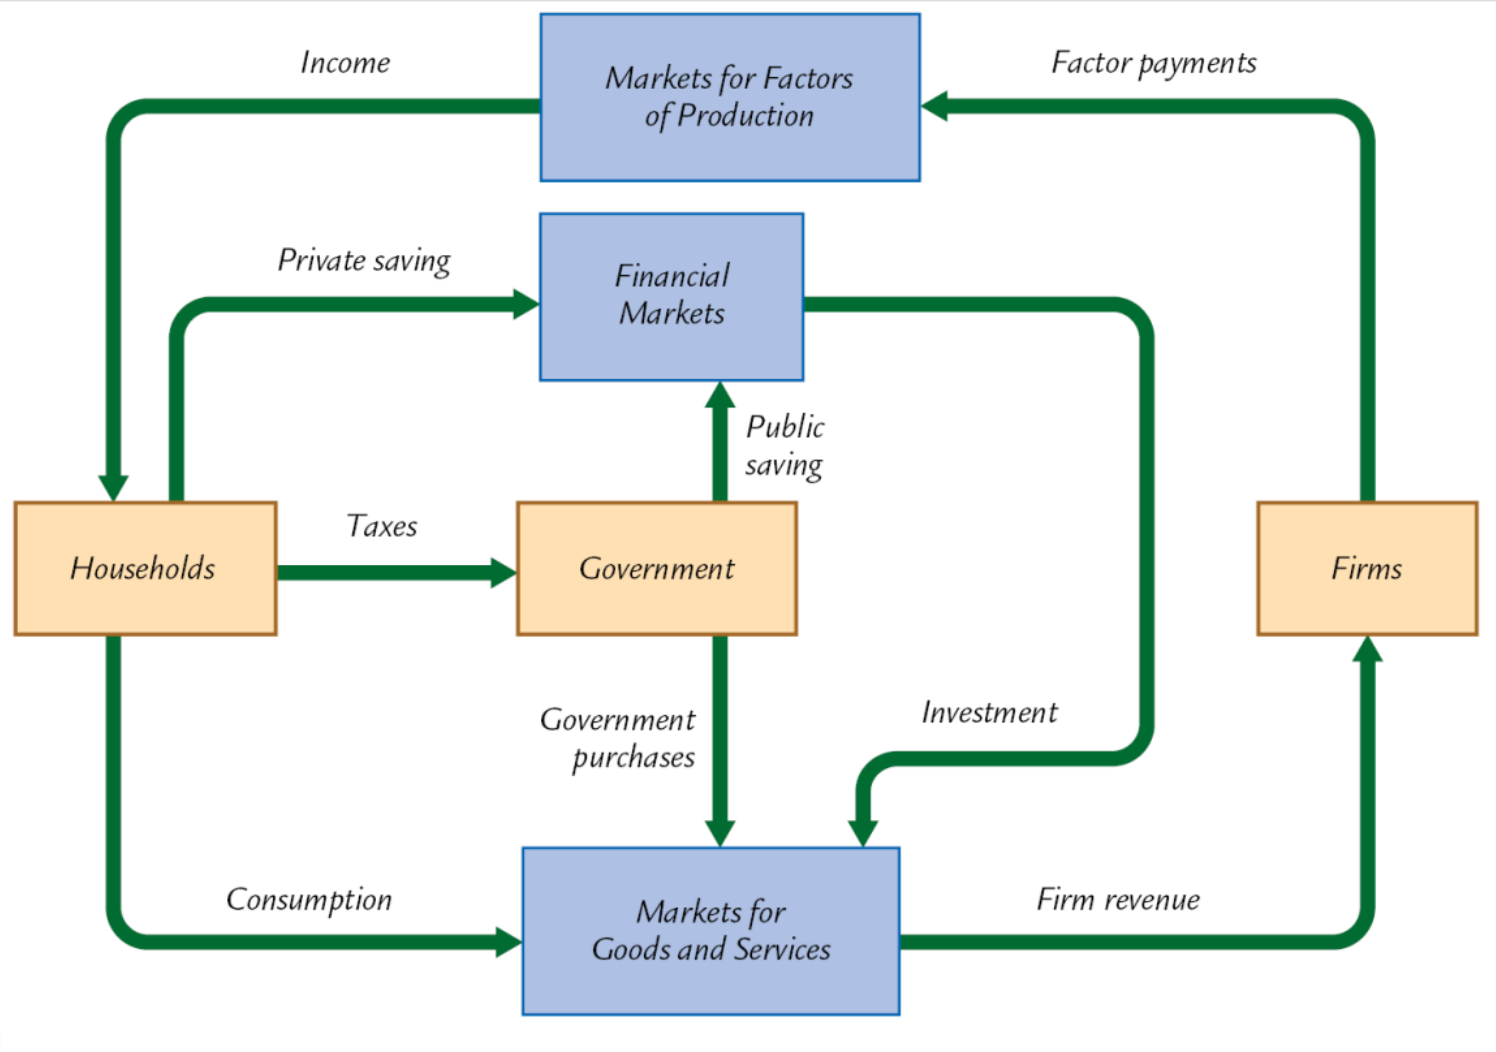
\includegraphics[width=0.8\textwidth]{image/RMBflow.png}
    \caption{经济中人民币的循环流动}
\end{figure}
\begin{itemize}
    \item 供给侧 
    \begin{itemize}
        \item 要素市场 (供给, 需求, 价格)
        \item 产出/收入的决定
    \end{itemize}
    \item 需求侧 
    \begin{itemize}
        \item C, I, G 的决定
    \end{itemize}
    \item 均衡
    \begin{itemize}
        \item goods market 商品市场
        \item loanable funds market 贷款市场
    \end{itemize}
\end{itemize}
\newpage
\section{The production function}
\begin{note}
    $K =$ captial 资本, $L =$ laber 劳动力, $Y = F(K, L)$ 生产函数
\end{note}
\begin{definition}
    对于 $Y_2 = F(zK, zL)$, $z > 1$, 
    \begin{itemize}
        \item constant returns to scale 规模报酬不变 : $zY_1 = Y_2$
        \item increasing returns to scale 递增规模报酬 : $zY_1 < Y_2$
        \item decreasing returns to scale 递减规模报酬 : $zY_1 > Y_2$
    \end{itemize}
\end{definition}
\begin{assumption}
    \begin{enumerate}
        \item 科技是固定的
        \item 经济体的资本劳动力供给是固定的, 分别为 $\overline{K}$ 和 $\overline{L}$ (充分就业, 资本充分利用)
        \item 资本和劳动力的边际产品是递减的
    \end{enumerate}
\end{assumption}
\begin{definition}
    \begin{itemize}
        \item W = Nominal wage 名义工资
        \item R = Nominal rental rate of capital 资本租金
        \item $P (= 1)$ = Price of output 产品价格
        \item $W/P$ = Real wage 实际工资
        \item $R/P$ = Real rental rate of capital 实际资本租金
    \end{itemize}
\end{definition}
\subsection{Demand for labor}
\begin{itemize}
    \item \textbf{假设市场是竞争性的}
    \begin{itemize}
        \item 每个企业将工资 $ W $、资本租金 $ R $ 和产品价格 $P $ 视为给定。
    \end{itemize}
    \item \textbf{基本思想}   
\begin{itemize}
        \item 企业雇佣每一单位劳动力的前提是成本不超过收益。
    \end{itemize}
    \item \textbf{成本与收益的衡量}
\begin{itemize}
        \item 成本 = 实际工资 $ \frac{W}{P} $
        \item 收益 = 劳动力的边际产出 $ MPL $
    \end{itemize}
\end{itemize}

\subsection{Marginal product of labor(MPL)}
\begin{definition}
    \textbf{MPL} = $\frac{\Delta Y}{\Delta L} = F(K,L+1)-F(K,L)$
\end{definition}
\begin{note}
    MPL 是劳动力的边际产品, 也是劳动力的边际收益.
\end{note}

\begin{figure}[htbp]
    \centering
    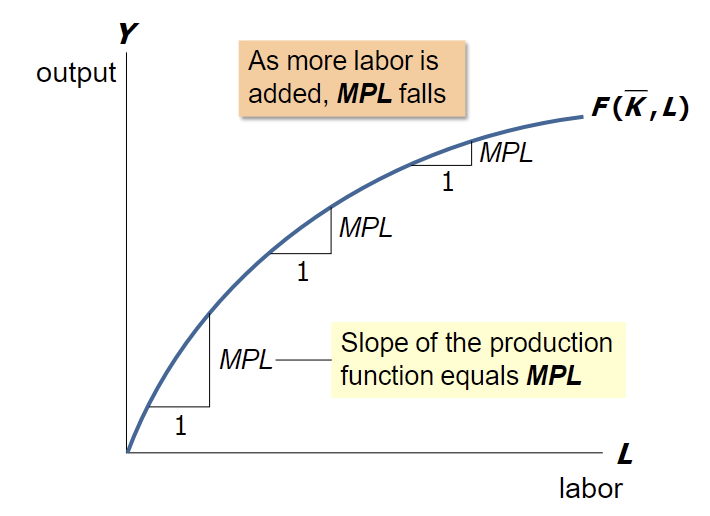
\includegraphics[width=0.7\textwidth]{image/MPLpf.png}
    \caption{边际产品和生产函数 : 边际递减}
\end{figure}


\begin{figure}[htbp]
    \centering
    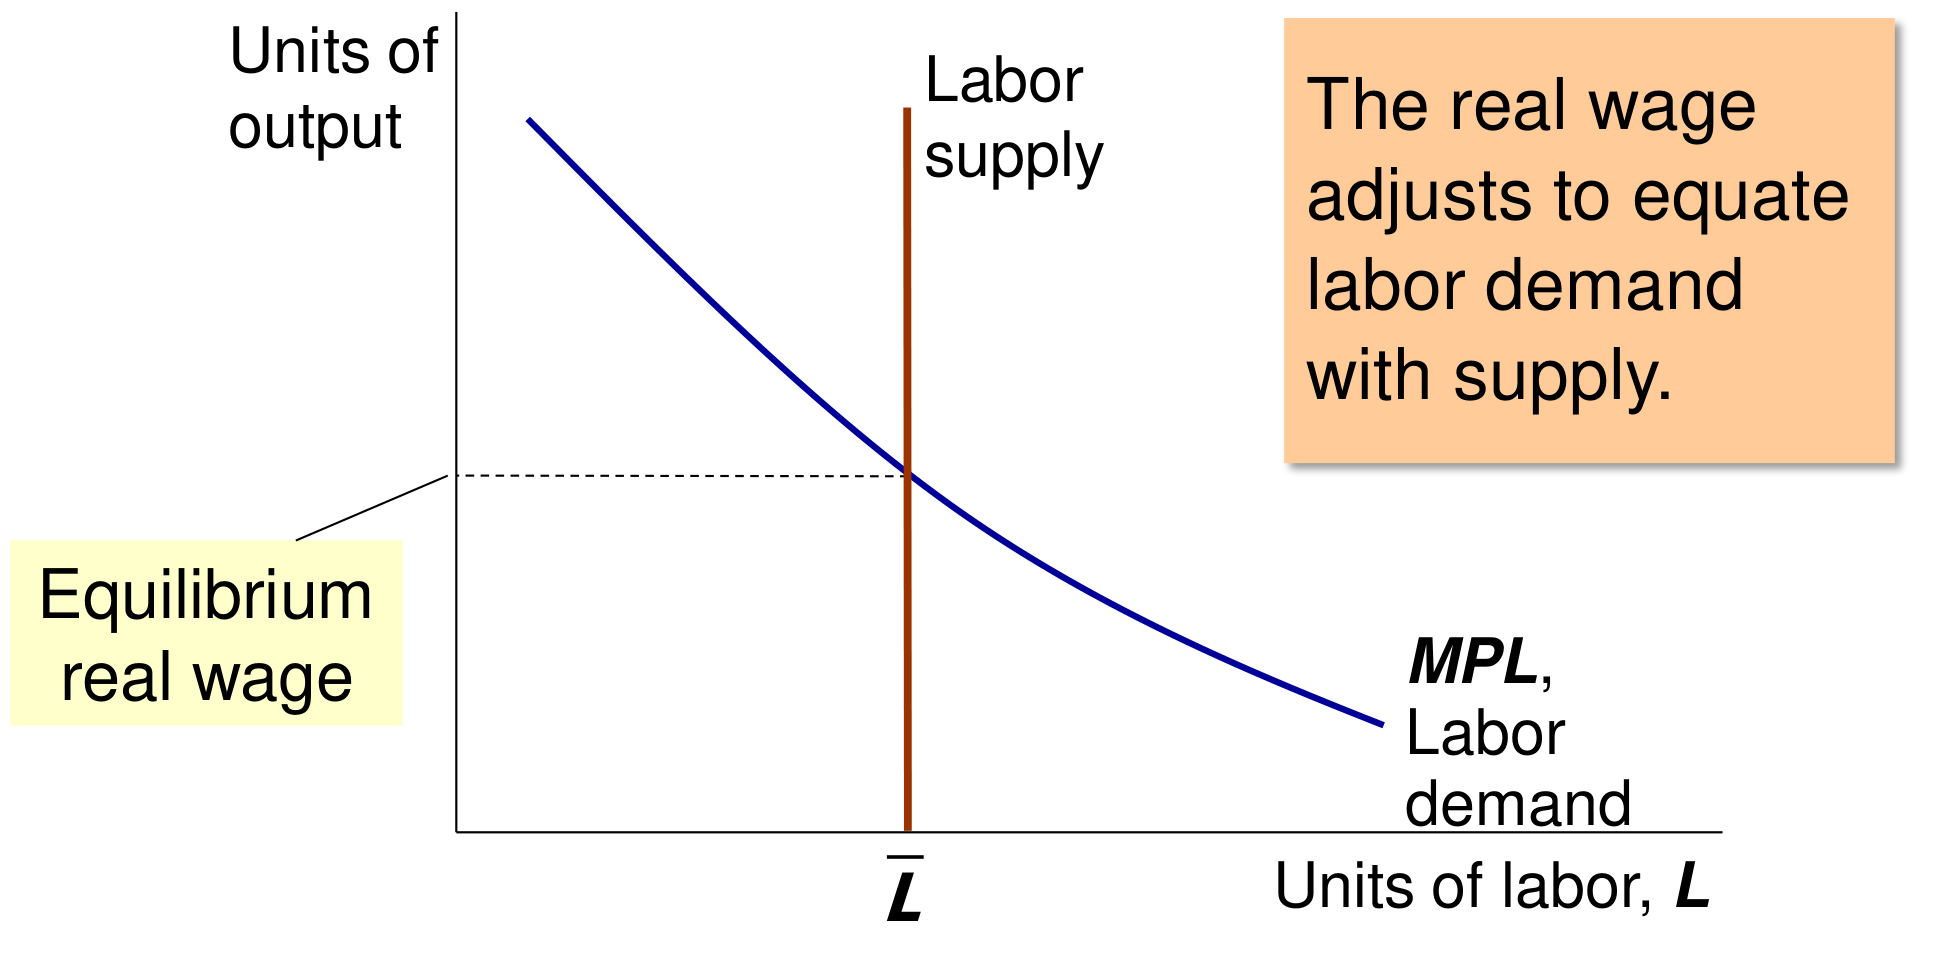
\includegraphics[width=0.7\textwidth]{image/equilibriumRW.png}
    \caption{均衡实际工资}
\end{figure}
\begin{figure}[htbp]
    \centering
    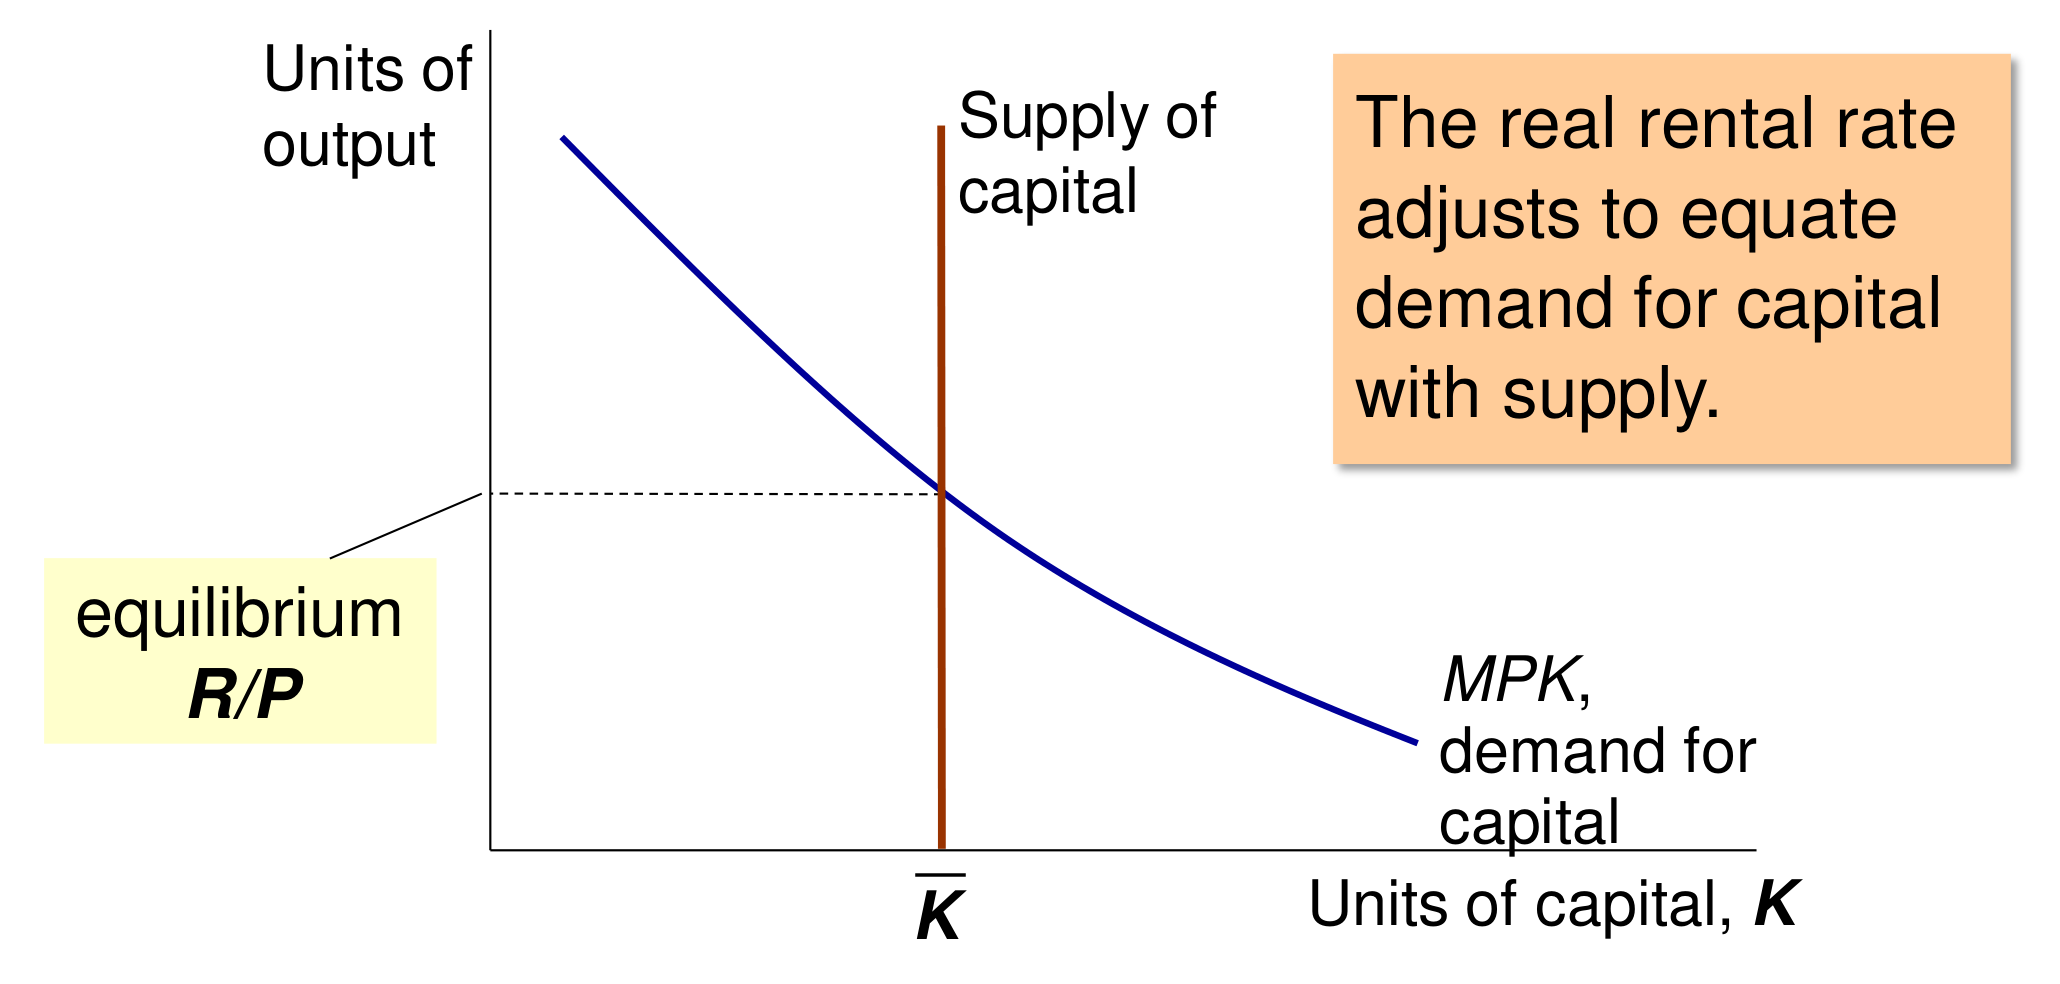
\includegraphics[width=0.7\textwidth]{image/equilibriumRRR.png}
    \caption{均衡实际租金}
\end{figure}
\begin{problem}
    How income is distributed among labor and capital
\end{problem}
\begin{itemize}
    \item Total labor income = $ \frac{W}{P}\overline{L}  = MPL \times \overline{L}$
    \item Total capital income = $ \frac{R}{P}\overline{K}  = MPK \times \overline{K}$
\end{itemize}
\begin{theorem}
    如果生成函数规模报酬不变, 则有: $$\overline{Y} = \overline{K} \times MPK + \overline{L} \times MPL$$
\end{theorem}

\subsection{The Cobb-Douglas production function}
\begin{definition}
    Cobb-Douglas 生产函数 : $Y = A \times K^{\alpha} \times L^{1-\alpha}$
\end{definition}
\begin{note}
    \begin{itemize}
        \item $A$ : total factor productivity 全要素生产率
        \item $\alpha$ : capital's share of income 资本收入份额
        \item $1-\alpha$ : labor's share of income 劳动力收入份额
    \end{itemize}
\end{note}
\begin{theorem}
    \begin{itemize}
        \item $MPK = \alpha \times \frac{Y}{K}$, 因为资本收入是 $MPK \times K$
        \item $MPL = (1-\alpha) \times \frac{Y}{L}$, 因为劳动力收入是 $MPL \times L$
    \end{itemize}
\end{theorem}
\begin{itemize}
    \item $Y/L$ : 平均劳动生产率
    \item $Y/K$ : 平均资本生产率
\end{itemize}

\subsection{收入不平等加剧的解释}
\begin{itemize}
    \item \textbf{资本收入份额的上升}
    \begin{itemize}
        \item 由于资本收入比劳动收入更加集中,资本收入份额的上升加剧了不平等。
    \end{itemize}

    \item \textbf{教育与技术的竞赛(Goldin \& Katz 的研究)}
    
\begin{itemize}
        \item 技术进步和全球化增加了对高技能工人相对于低技能工人的需求。
        \item 由于教育扩张速度放缓,高技能工人的供给未能跟上需求。
        \item 结果:高技能工人与低技能工人之间的工资差距扩大。
    \end{itemize}
\end{itemize}

\section{Demand for goods and services}

\begin{itemize}
    \item C = consumer demand for g\& s
    \item I = demand for investment goods
    \item G = government demand for g\& s
    \item closed economy : no NX
\end{itemize}

\newpage

\subsection{Consumption}
\begin{figure}[htbp]
    \centering
    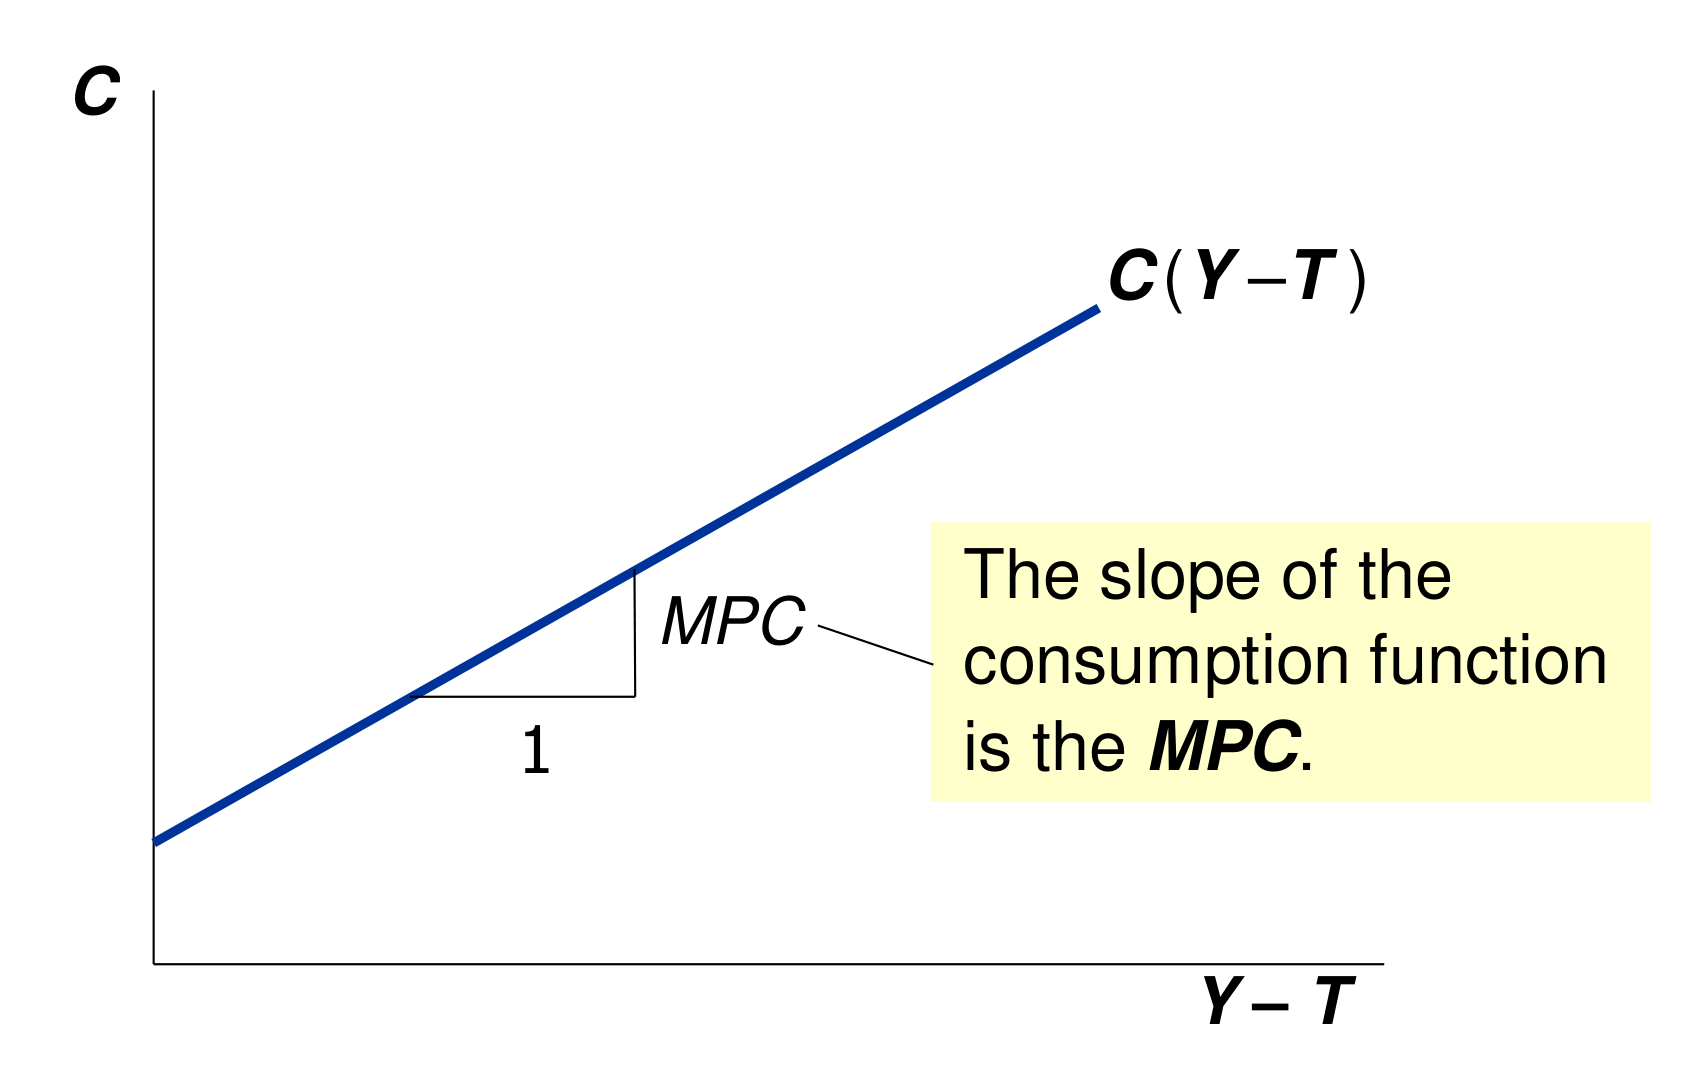
\includegraphics[width=0.7\textwidth]{image/ConsumptionFunction.png}
    \caption{消费函数}
\end{figure}
\begin{itemize}
    \item \textbf{可支配收入} 是总收入减去总税收:$Y - T$。
    \item 消费函数:$C = C (Y - T )$
    \item 定义:\textbf{边际消费倾向 (MPC)} 是指可支配收入增加一美元时,消费 $C$ 的变化量。
\end{itemize}

\subsection{Investment}
\begin{figure}[htbp]
    \centering
    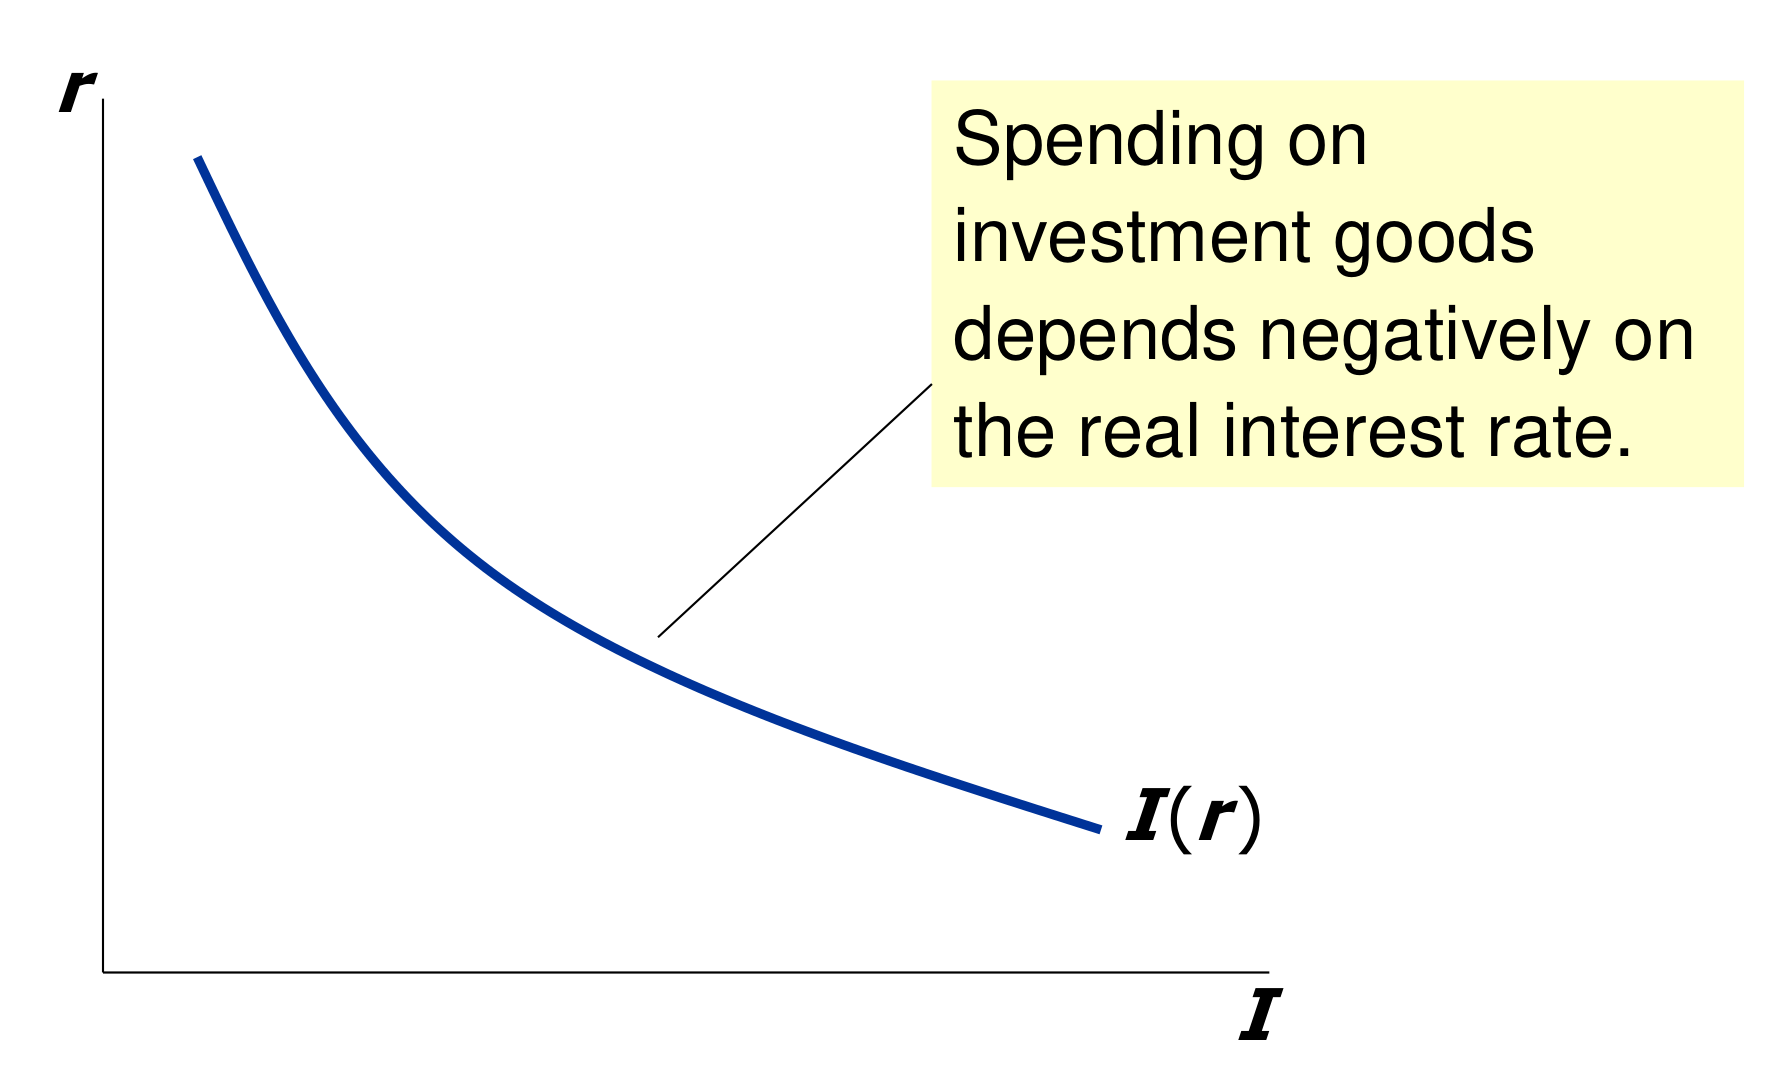
\includegraphics[width=0.7\textwidth]{image/Investmentfunction.png}
    \caption{投资函数}
\end{figure}
\begin{itemize}
    \item 投资函数为
    $
    I = I(r)
    $
    , 其中 $ r $表示实际利率,即经过通胀调整后的名义利率。
    
    \item 实际利率是:
    \begin{itemize}
        \item 借贷的成本
        \item 使用自有资金进行投资的机会成本
    \end{itemize}
    
    \item 因此,$ I $ 与 $ r $ 负相关。
\end{itemize}
\subsection{Government spending}
\begin{itemize}
    \item $G$ = 政府在商品和服务上的支出
    \item $G$ 不包括转移支付(例如,社会保障福利、失业保险福利)
    \item 假设政府支出和总税收是外生的:$G = G$ 且 $T = T$
\end{itemize}

\begin{proposition}[商品和服务市场]
    \begin{itemize}
        \item 总需求:
        $$
        Y = C(Y - T) + I(r) + G
        $$
        \item 总供给:
        $$
        Y = F(K, L)
        $$
        \item 均衡:
        $$
        Y = C(Y - T) + I(r) + G
        $$
        \item 实际利率调整以使需求等于供给:
    \end{itemize}
\end{proposition}

\newpage

\section{The loanable funds market}
\begin{itemize}
    \item 信贷市场 : 金融系统的简单供需模型。
    \item 一种资产:“信贷”
    \begin{itemize}
        \item 资金需求:投资
        \item 资金供给:储蓄
        \item 资金的“价格”:实际利率
    \end{itemize}
    \item 对信贷的需求
    \begin{itemize}
        \item 投资者希望借入资金以进行投资
        \item 投资者的需求曲线是向下倾斜的
    \end{itemize}
\end{itemize}
\begin{note}
    信贷市场的投资曲线和之前的投资函数是一样的.
\end{note}

\begin{definition}[储蓄的类型]
    \begin{itemize}
        \item 私人储蓄:$= (Y - T) - C$
        \item 公共储蓄:$= T - G$
        \item 总储蓄(National saving):$S = (Y - T) - C + T - G = Y - C - G$
    \end{itemize}
\end{definition}

\begin{definition}[预算盈余和赤字]
    \begin{itemize}
        \item 预算盈余:$T - G = $ 公共储蓄
        \item 赤字:$G - T$
        \item 如果 $G = T$, 预算平衡 (balanced budget)
    \end{itemize}
\end{definition}
\begin{note} 美国政府通过发行国债来为其赤字提供资金, 也就是借. 实际上高债务是一个全球现象, \end{note}
\begin{figure}[htbp]
    \centering
    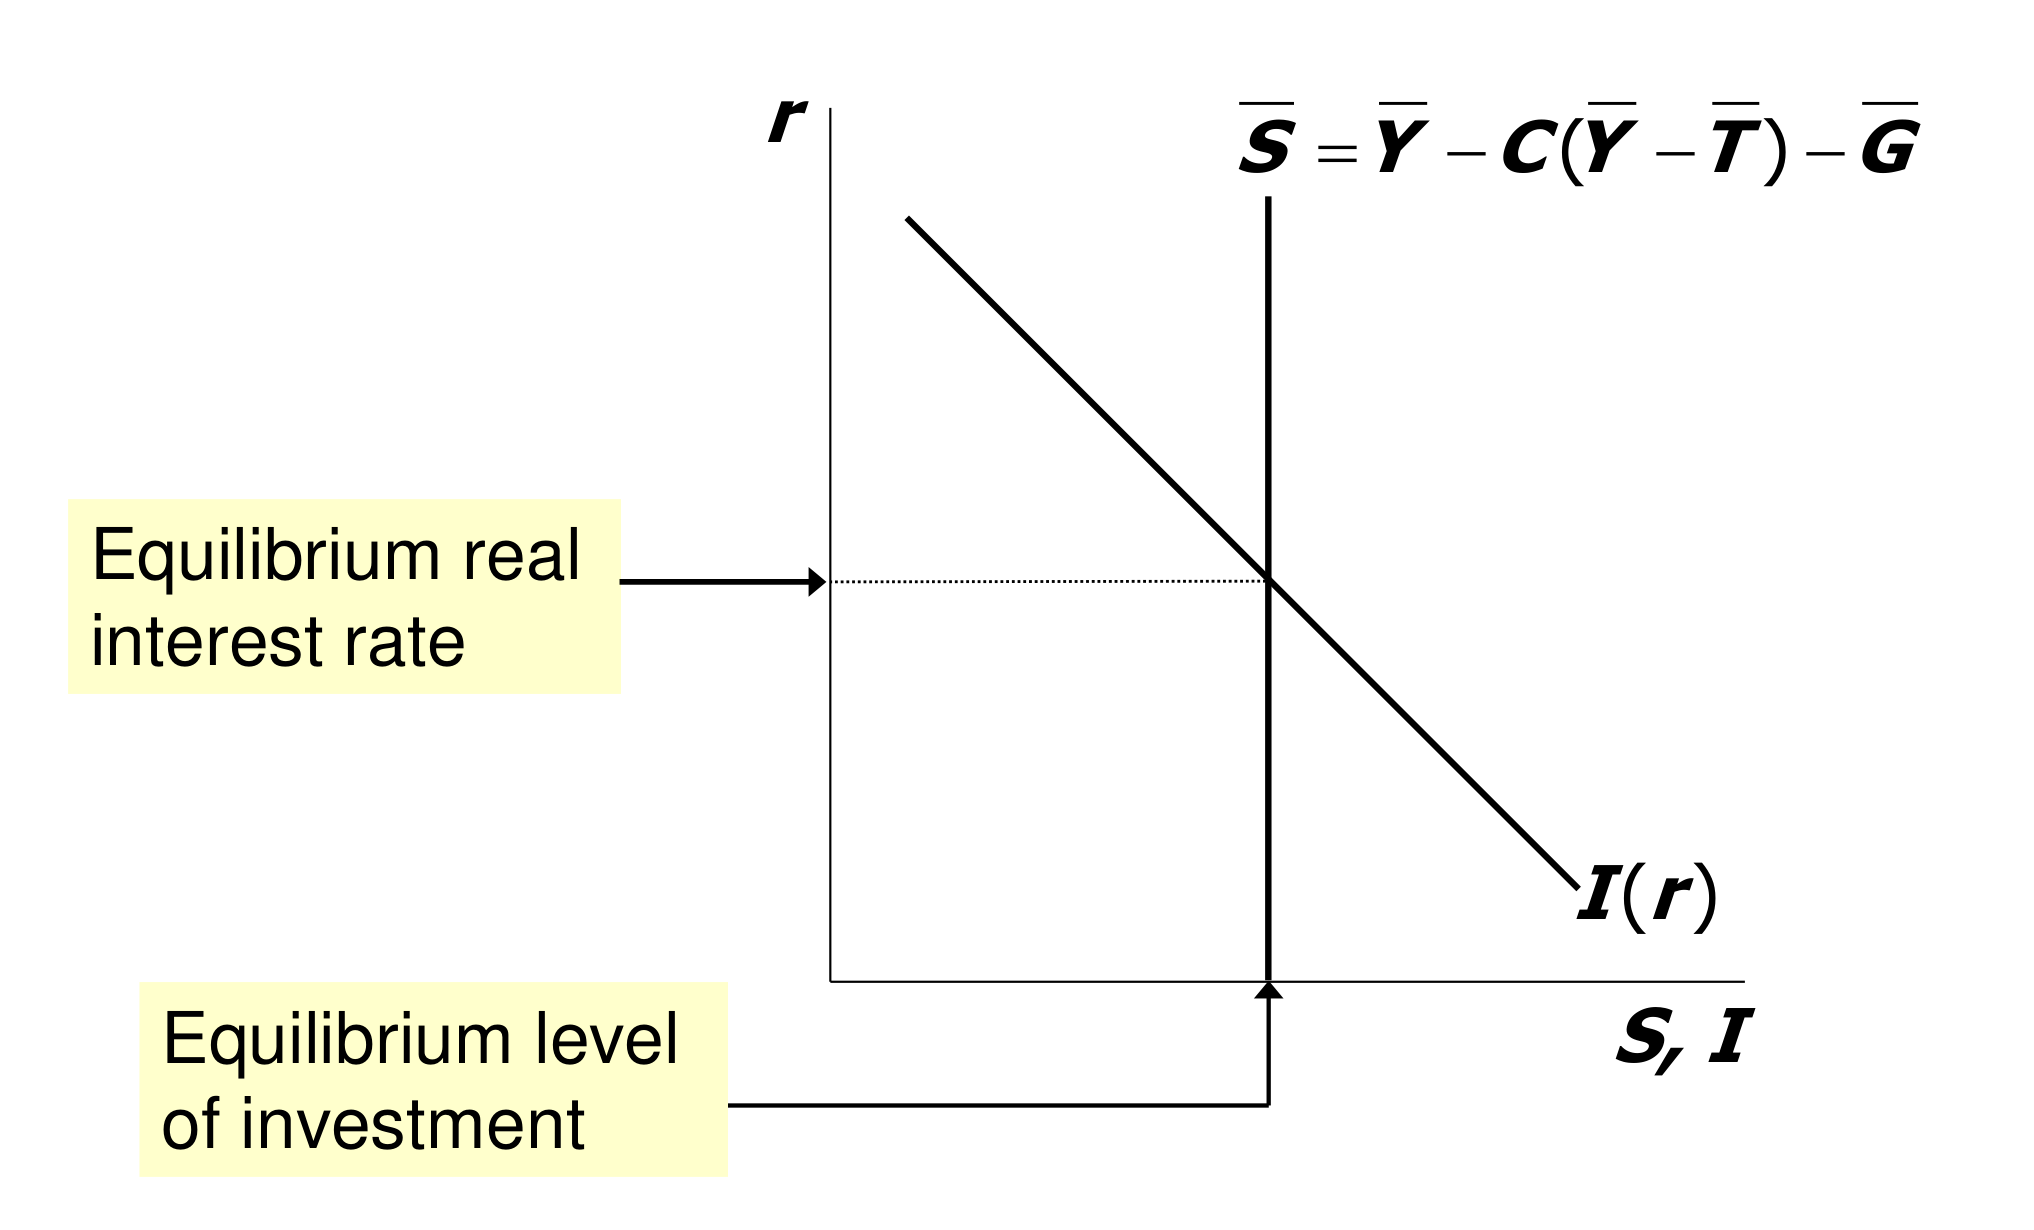
\includegraphics[width=0.7\textwidth]{image/Loanablefundsmarketequilibrium.png}
    \caption{信贷市场均衡}
\end{figure}

\begin{note} 本节最后以信贷市场为案例讲了一些比较静态分析, 或者说去 mastering 某个变化 (例如政府增大支出且减税) 带来的影响 (减少储蓄), 不再赘述 
    
政府增大支出可能来自于新冠疫情等 \end{note}

%\end{document}
